\documentclass[11pt]{article}
\usepackage[dvipsnames]{xcolor}
\usepackage{tikz}
\usetikzlibrary{arrows, shapes, positioning}
\usepackage{pgfmath}
\usepackage{setspace}
\usepackage{amsmath}
\usepackage{array}
\usepackage{hyperref}
\usepackage{enumerate}
\usepackage{enumitem}
\setlist{noitemsep}
\usepackage{listings}
\lstset{language=python}
\usepackage{makeidx}
\usepackage{verbatim}
\usepackage{datetime}

\setlength{\pdfpageheight}{11in}
\setlength{\textheight}{9in}
\setlength{\voffset}{-1in}
\setlength{\oddsidemargin}{0pt}
\setlength{\marginparsep}{0pt}
\setlength{\marginparwidth}{0pt}
\setlength{\marginparpush}{0pt}
\setlength{\textwidth}{6.5in}

\pagestyle{plain}
\makeindex

\title{Crash Test Data Exploration}
\author{Brad Burkman}
\newdateformat{vardate}{\THEDAY\ \monthname[\THEMONTH]\ \THEYEAR}
\vardate
\date{\today}

\begin{document}
\setlength{\parindent}{20pt}
\begin{spacing}{1.2}
\maketitle

%%%%%%%%%%%
\section{Introduction}

%%%
\subsection{Goal}

Given the \verb|2019 Crash 1 Database.csv| from Dr. XiaoDuan Sun and her student Malek Abuhijeh, I'm trying different machine learning algorithms to make sense of the data.  

%%%
\subsection{Initial Question}

Of the many factors in each crash, and the range of values for those factors, which ones most heavily correlate to the crash being fatal?

%%%
\subsection{Requisite Nerdy Image of Negligible Relevance}

\

\includegraphics[width=4in]{Mountain_Lion.png}

\tableofcontents

\section{Data}

The data was 160,186 records of crashes in Louisiana in 2019, with 79 fields per record.  Some of the fields had a reasonable number of unique elements, like , like ``Principal Contributing Factor'' with thirteen unique values (and blank and ``1,'' which didn't seem to mean anything), but others had many different elements, like ``Principal Road Name.''  Presuming that we were more likely to find strong correlations in fields with a small number of unique values, I arbitrarily chose twenty unique values as the cutoff, tossing out the fields with more variety.  

I used one-hot encoding to make each of the 415 remaining unique values into its own $\{0,1\}$ vector.


\section{Tools}

I will start with scikit-learn, and work through its machine learning algorithm selection diagram.  

\noindent\includegraphics[width=6.5in]{ml_map.png}

\section{First Try: SGD Regressor}

We're going to treat the severity of the accident as a real number in $[0,1]$.  The raw data set gives the severity in five categories, which we will convert to a real number.

\

\hfil\begin{tabular}{llll}
	Description & Raw Data & Feature-Engineered Data \cr\hline
	FATAL & A & 0.9 \cr
	SEVERE & B & 0.7 \cr
	MODERATE & C & 0.5 \cr
	COMPLAINT & D & 0.3 \cr
	NO INJURY & E & 0.1 \cr
\end{tabular}

\

The scikit-learn machine learning algorithm cheat sheet says the Stochastic Gradient Descent (SGD) Regressor algorithm is appropriate.  We can also use SGDClassifier if we treat ``FATAL'' as $1$ and the others as $-1$.

\

\hfil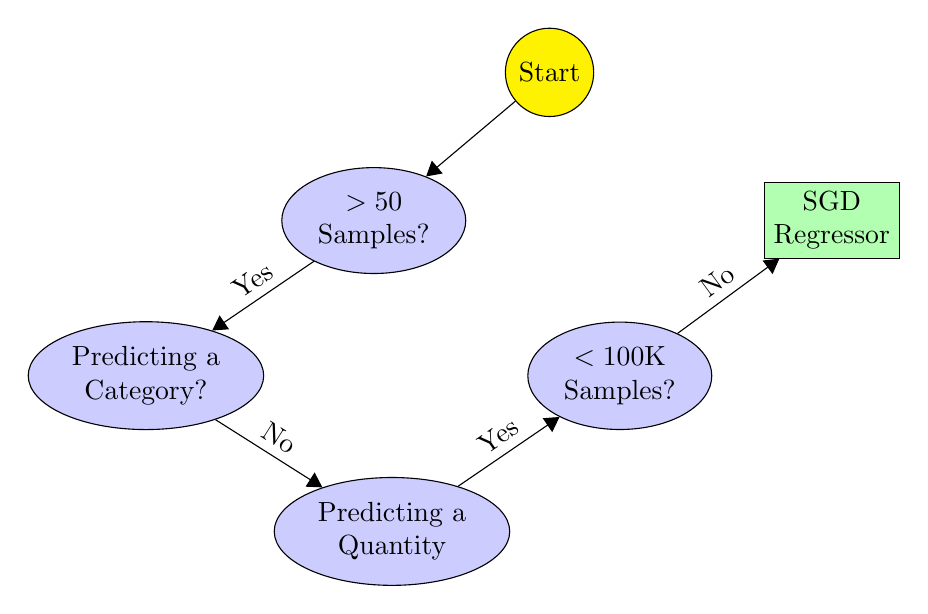
\begin{tikzpicture}[]
	\node [draw, circle, fill = yellow] (Start) at (0,0) [] {Start};
	\node [draw, ellipse, fill=white!80!blue, align=center, below left = of Start] (Fifty) {$>50$ \\ Samples?}; 
	\node [draw, ellipse, fill=white!80!blue, align=center, below left = of Fifty] (Category) {Predicting a \\ Category?};
	\node [draw, ellipse, fill=white!80!blue, align=center, below right = of Category] (Quantity) {Predicting a \\ Quantity};
	\node [draw, ellipse, fill=white!80!blue, align=center, above right = of Quantity] (100K) {$<100$K \\ Samples?};
	\node [draw, rectangle, fill=white!70!green, align=center, above right = of 100K] (SGD Regressor) {SGD \\ Regressor};
	\draw [-triangle 60] (Start) -- (Fifty);
	\draw [-triangle 60] (Fifty) -- (Category) node [midway, sloped, above] {Yes};
	\draw [-triangle 60] (Category) -- (Quantity) node [midway, sloped, above] {No};
	\draw [-triangle 60] (Quantity) -- (100K) node [midway, sloped, above] {Yes};
	\draw [-triangle 60] (100K) -- (SGD Regressor) node [midway, sloped, above] {No};
%	\draw [-triangle 60] () -- () node [midway, sloped, above] {};
%	\node [draw, ellipse, align=center, ] () {};
\end{tikzpicture}


\section{Output, Trying to Understand Linear Coefficients}

It makes sense that the number of people killed in the accident being zero would negatively correlate with the accident being fatal, and there being more fatal crashes with one death than four, so the coefficients seem to be ordered according to our expectations.  

\

\qquad\begin{tabular}{rrrr}
\verb|coef_| & Category & Value & Key \cr\hline
0.1585 & \verb|num_tot_kil| & 1 &  \cr
0.0163 & \verb|num_tot_kil| & 2 &  \cr
0.0039 & \verb|num_tot_kil| & 3 &  \cr
0.0005 & \verb|num_tot_kil| & 4 &  \cr
-0.1299 & \verb|num_tot_kil| & 0 &  \cr\cline{1-1}
0.0493 & \verb|num_tot_kil| & Sum &  \cr \end{tabular}
 
 \
 
 It makes sense that head-on collisions would be most fatal, and left turns more deadly than right.  
 
 \
 
\qquad\begin{tabular}{rrrl}
\verb|coef_| & Category & Value & Key \cr\hline
0.0049 & \verb|man_coll_cd| & C & HEAD-ON \cr
0.0042 & \verb|man_coll_cd| & A & NON-COLLISION WITH MOTOR VEHICLE \cr
0.0042 & \verb|man_coll_cd| & J & SIDESWIPE - SAME DIRECTION \cr
0.0042 & \verb|man_coll_cd| & B & REAR END \cr
0.0042 & \verb|man_coll_cd| & Z & OTHER \cr
0.0041 & \verb|man_coll_cd| & K & SIDESWIPE - OPPOSITE DIRECTION \cr
0.0041 & \verb|man_coll_cd| & G & LEFT TURN - SAME DIRECTION \cr
0.0041 & \verb|man_coll_cd| & E & LEFT TURN - ANGLE \cr
0.0041 & \verb|man_coll_cd| & D & RIGHT ANGLE \cr
0.0041 & \verb|man_coll_cd| & F & LEFT TURN - OPPOSITE DIRECTION \cr
0.0040 & \verb|man_coll_cd| & H & RIGHT TURN - SAME DIRECTION \cr
0.0031 & \verb|man_coll_cd| & I & RIGHT TURN - OPPOSITE DIRECTION \cr\cline{1-1}
0.0493 & \verb|man_coll_cd| & Sum &  \cr
\end{tabular}

\

This one also satisfies expectations, because while snowy and icy conditions are dangerous, they are rare in Louisiana.  

\

\qquad\begin{tabular}{rrrl}
\verb|coef_| & Category & Value & Key \cr\hline
0.0115 & \verb|surf_cond_cd| & B & WET \cr
0.0114 & \verb|surf_cond_cd| & A & DRY \cr
0.0100 & \verb|surf_cond_cd| & Y & UNKNOWN \cr
0.0052 & \verb|surf_cond_cd| & 2 &  \cr
0.0031 & \verb|surf_cond_cd| & D & ICE \cr
0.0029 & \verb|surf_cond_cd| &  &  \cr
0.0026 & \verb|surf_cond_cd| & E & CONTAMINANT (SAND, MUD, DIRT, OIL, ETC.) \cr
0.0012 & \verb|surf_cond_cd| & Z & OTHER \cr
0.0008 & \verb|surf_cond_cd| & C & SNOW/SLUSH \cr
0.0007 & \verb|surf_cond_cd| & 1 &  \cr\cline{1-1}
0.0493 & \verb|surf_cond_cd| & Sum &  \cr
\end{tabular}

\

The driver's age doesn't seem to be correlated with the severity of the accident.  Note that I changed the ages from years to decades to get fewer distinct values.  Many records list the age as 200 years.  (?)

\

\qquad\begin{tabular}{rrrr}
\verb|coef_| & Category & Value & Key \cr\hline
0.0051 & \verb|dr_age_1| & 80 &  \cr
0.0051 & \verb|dr_age_1| & 70 &  \cr
0.0051 & \verb|dr_age_1| & 10 &  \cr
0.0050 & \verb|dr_age_1| & 30 &  \cr
0.0050 & \verb|dr_age_1| & 40 &  \cr
0.0050 & \verb|dr_age_1| & 60 &  \cr
0.0050 & \verb|dr_age_1| & 50 &  \cr
0.0050 & \verb|dr_age_1| & 20 &  \cr
0.0042 & \verb|dr_age_1| & 90 &  \cr
0.0038 & \verb|dr_age_1| & 200 &  \cr
0.0008 & \verb|dr_age_1| & 0 &  \cr
0.0002 & \verb|dr_age_1| &  &  \cr
0.0000 & \verb|dr_age_1| & 110 &  \cr
0.0000 & \verb|dr_age_1| & 100 &  \cr\cline{1-1}
0.0493 & \verb|dr_age_1| & Sum &  \cr
\end{tabular}

\

The driver's gender also doesn't seem to play a role.  

\

\qquad\begin{tabular}{rrrr}
\verb|coef_| & Category & Value & Key \cr\hline
0.0165 & \verb|dr_sex_1| &  &  \cr
0.0165 & \verb|dr_sex_1| & M &  \cr
0.0164 & \verb|dr_sex_1| & F &  \cr\cline{1-1}
0.0493 & \verb|dr_sex_1| & Sum &  \cr
\end{tabular}

\section{Deflated Hopes}

I had hoped that the sum of the coefficients for each category would be different, indicating which categories were had the strongest correlation to the severity of the accident, but they're all the same.  

\section{Request}

Can you recommend a source I can read that will explain how to interpret the results?  I emailed Henry, who taught me to use scikit-learn, but I have not heard back.  

Thank you!

%%%%%%%%%%%%%%%%%%
% Index
\clearpage
\addcontentsline{toc}{section}{Index}
\printindex

%%%%%%%%%%%%%%%%
\end{spacing}
\end{document}

%%%%%%%%%%%%
% Useful tools
%%%%%%%%%

\begin{lstlisting}
Put your code here.
\end{lstlisting}

\lstinputlisting[language=python]{source_filename.py}


